\documentclass{standalone}
\usepackage{tikz}
\usetikzlibrary{
  arrows,
  calc,
  decorations.pathmorphing,
  decorations.pathreplacing,
  decorations.markings,
  fadings,
  positioning,
  shapes,
  arrows.meta
}
\pgfdeclareradialshading{glow}{\pgfpoint{0cm}{0cm}}{
  color(0mm)=(white);
  color(5mm)=(white);
  color(9mm)=(black);
  color(10mm)=(black)
}

\begin{tikzfadingfrompicture}[name=glow fading]
  \shade [shading=glow] (0,0) circle (1);
\end{tikzfadingfrompicture}

\ifpdf
% Ensure reproducible output
\pdfinfoomitdate=1
\pdfsuppressptexinfo=-1
\pdftrailerid{}
\fi

\begin{document}

\begin{tikzpicture}[scale=1.3593]
  % f_pa0 = 288711.765(84) GHz
  % offset_3 = 770.204520(60) MHz
  % offset_6 = 770.20805(12) MHz
  % offset_15 = 770.19429(29) MHz
  % slope_3 = -12.459(17) MHz GHz
  % slope_6 = -24.444(32) MHz GHz
  % slope_15 = -60.660(80) MHz GHz

  % offset^0 = 770.19693(24) MHz
  % offset^1 = 3.208(88) kHz / mW
  % offset^2 = -0.2256(53) kHz / mW^2
  % slope^1 = -4.0887(31) MHz GHz / mW
  \node at (-0.1cm - 1pt, 0) {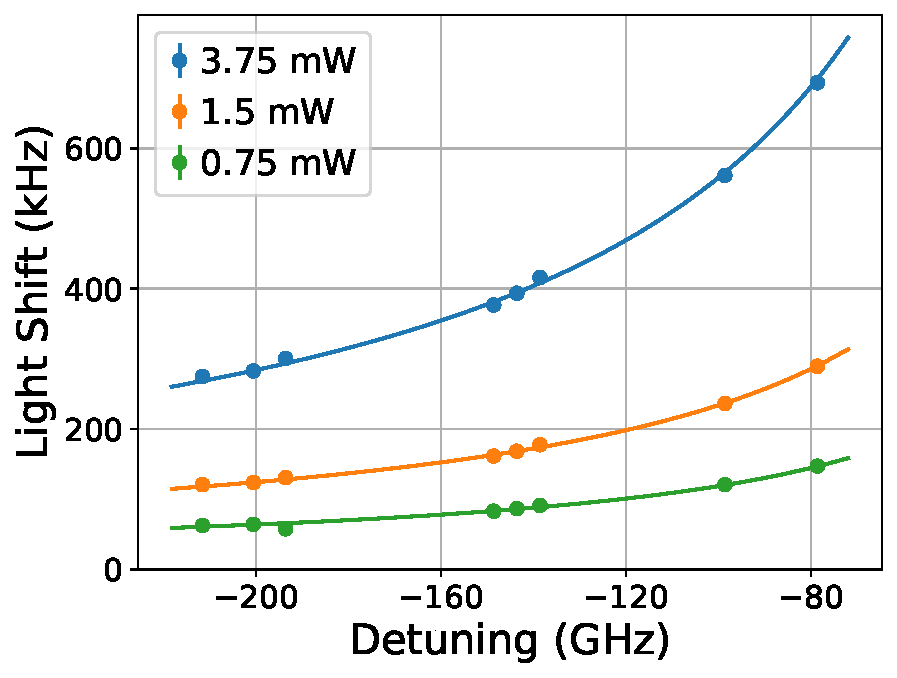
\includegraphics[height=4.7577cm]{scaling_light_shift.pdf}};
  \node at (-2.0cm - 1pt, 1.5) {\footnotesize (\textbf{a})};

  % offset_3 = -2pi 0.293(23) kHz
  % offset_6 = -2pi 0.631(44) kHz
  % offset_15 = -2pi 2.46(15) kHz
  % slope_3 = -4pi^2 115.4(39) kHz GHz
  % slope_6 = -4pi^2 274.7(59) kHz GHz
  % slope_15 = -4pi^2 952(25) kHz GHz

  % offset^1.29 = -2pi 68.9(27) Hz/mW^-1.29
  % slope^1.29 = -4pi^2 27.88(41) kHz GHz/mW^-1.29
  \node at (4.45, 0) {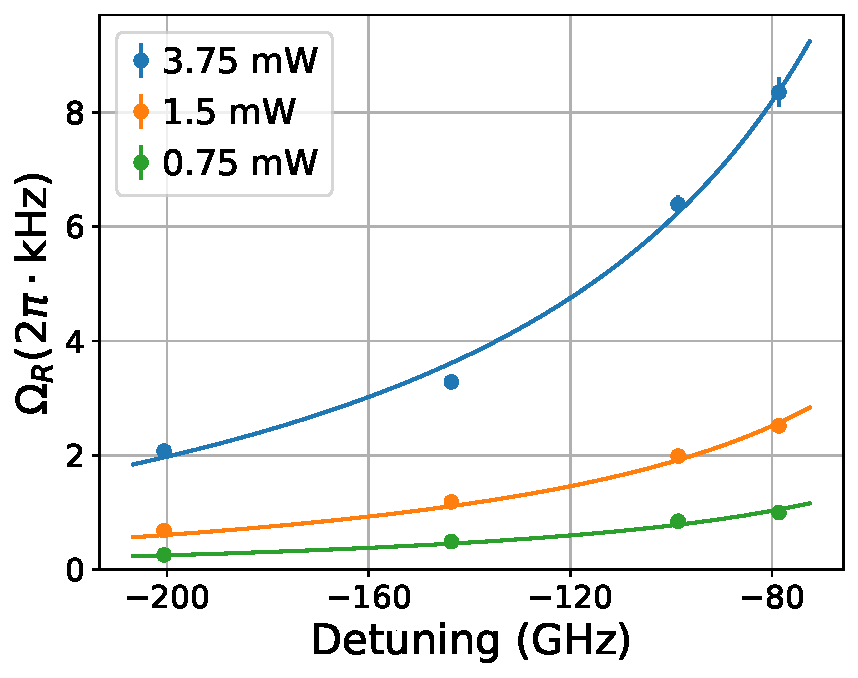
\includegraphics[height=4.7577cm]{scaling_rabi.pdf}};
  \node at (2.5, 1.5) {\footnotesize (\textbf{b})};

  % omega_m: 2pi 90.434(34) MHz/mW^0.5
  % omega_a: 2pi 617.1(92) kHz/mW^0.79
  \node at (8.1cm + 1pt, 0) {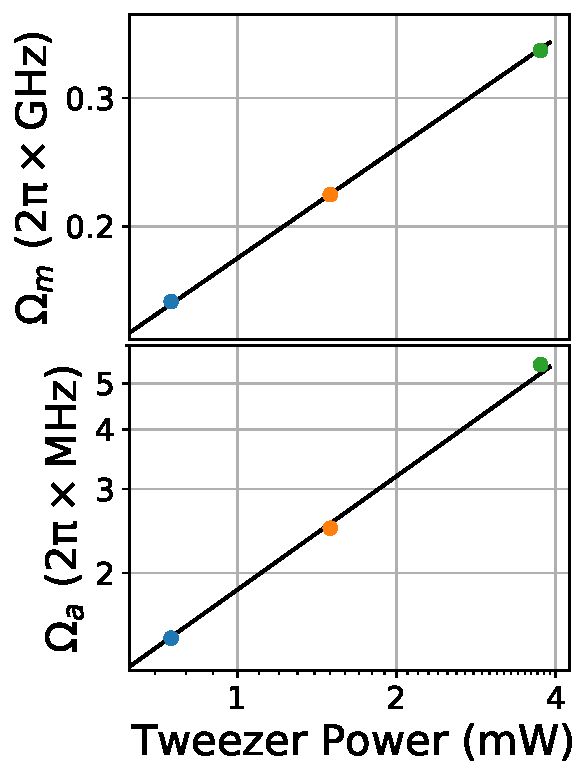
\includegraphics[height=5.0296cm]{scaling_slopes.pdf}};
  \node at (7.6cm + 1pt, 1.55) {\footnotesize (\textbf{c})};
\end{tikzpicture}

\end{document}
